\task{Разрезания}
\begin{enumerate}
\itA Укажите, как разрезать произвольный квадрат на 7 многоугольников, у которых одинаковы как площади, так и суммарные длины сторон, лежащих на границе исходного квадрата.

\itB Укажите, как разрезать изображённую на рисунке 2 фигуру на 6 равных фигур.

\centerline{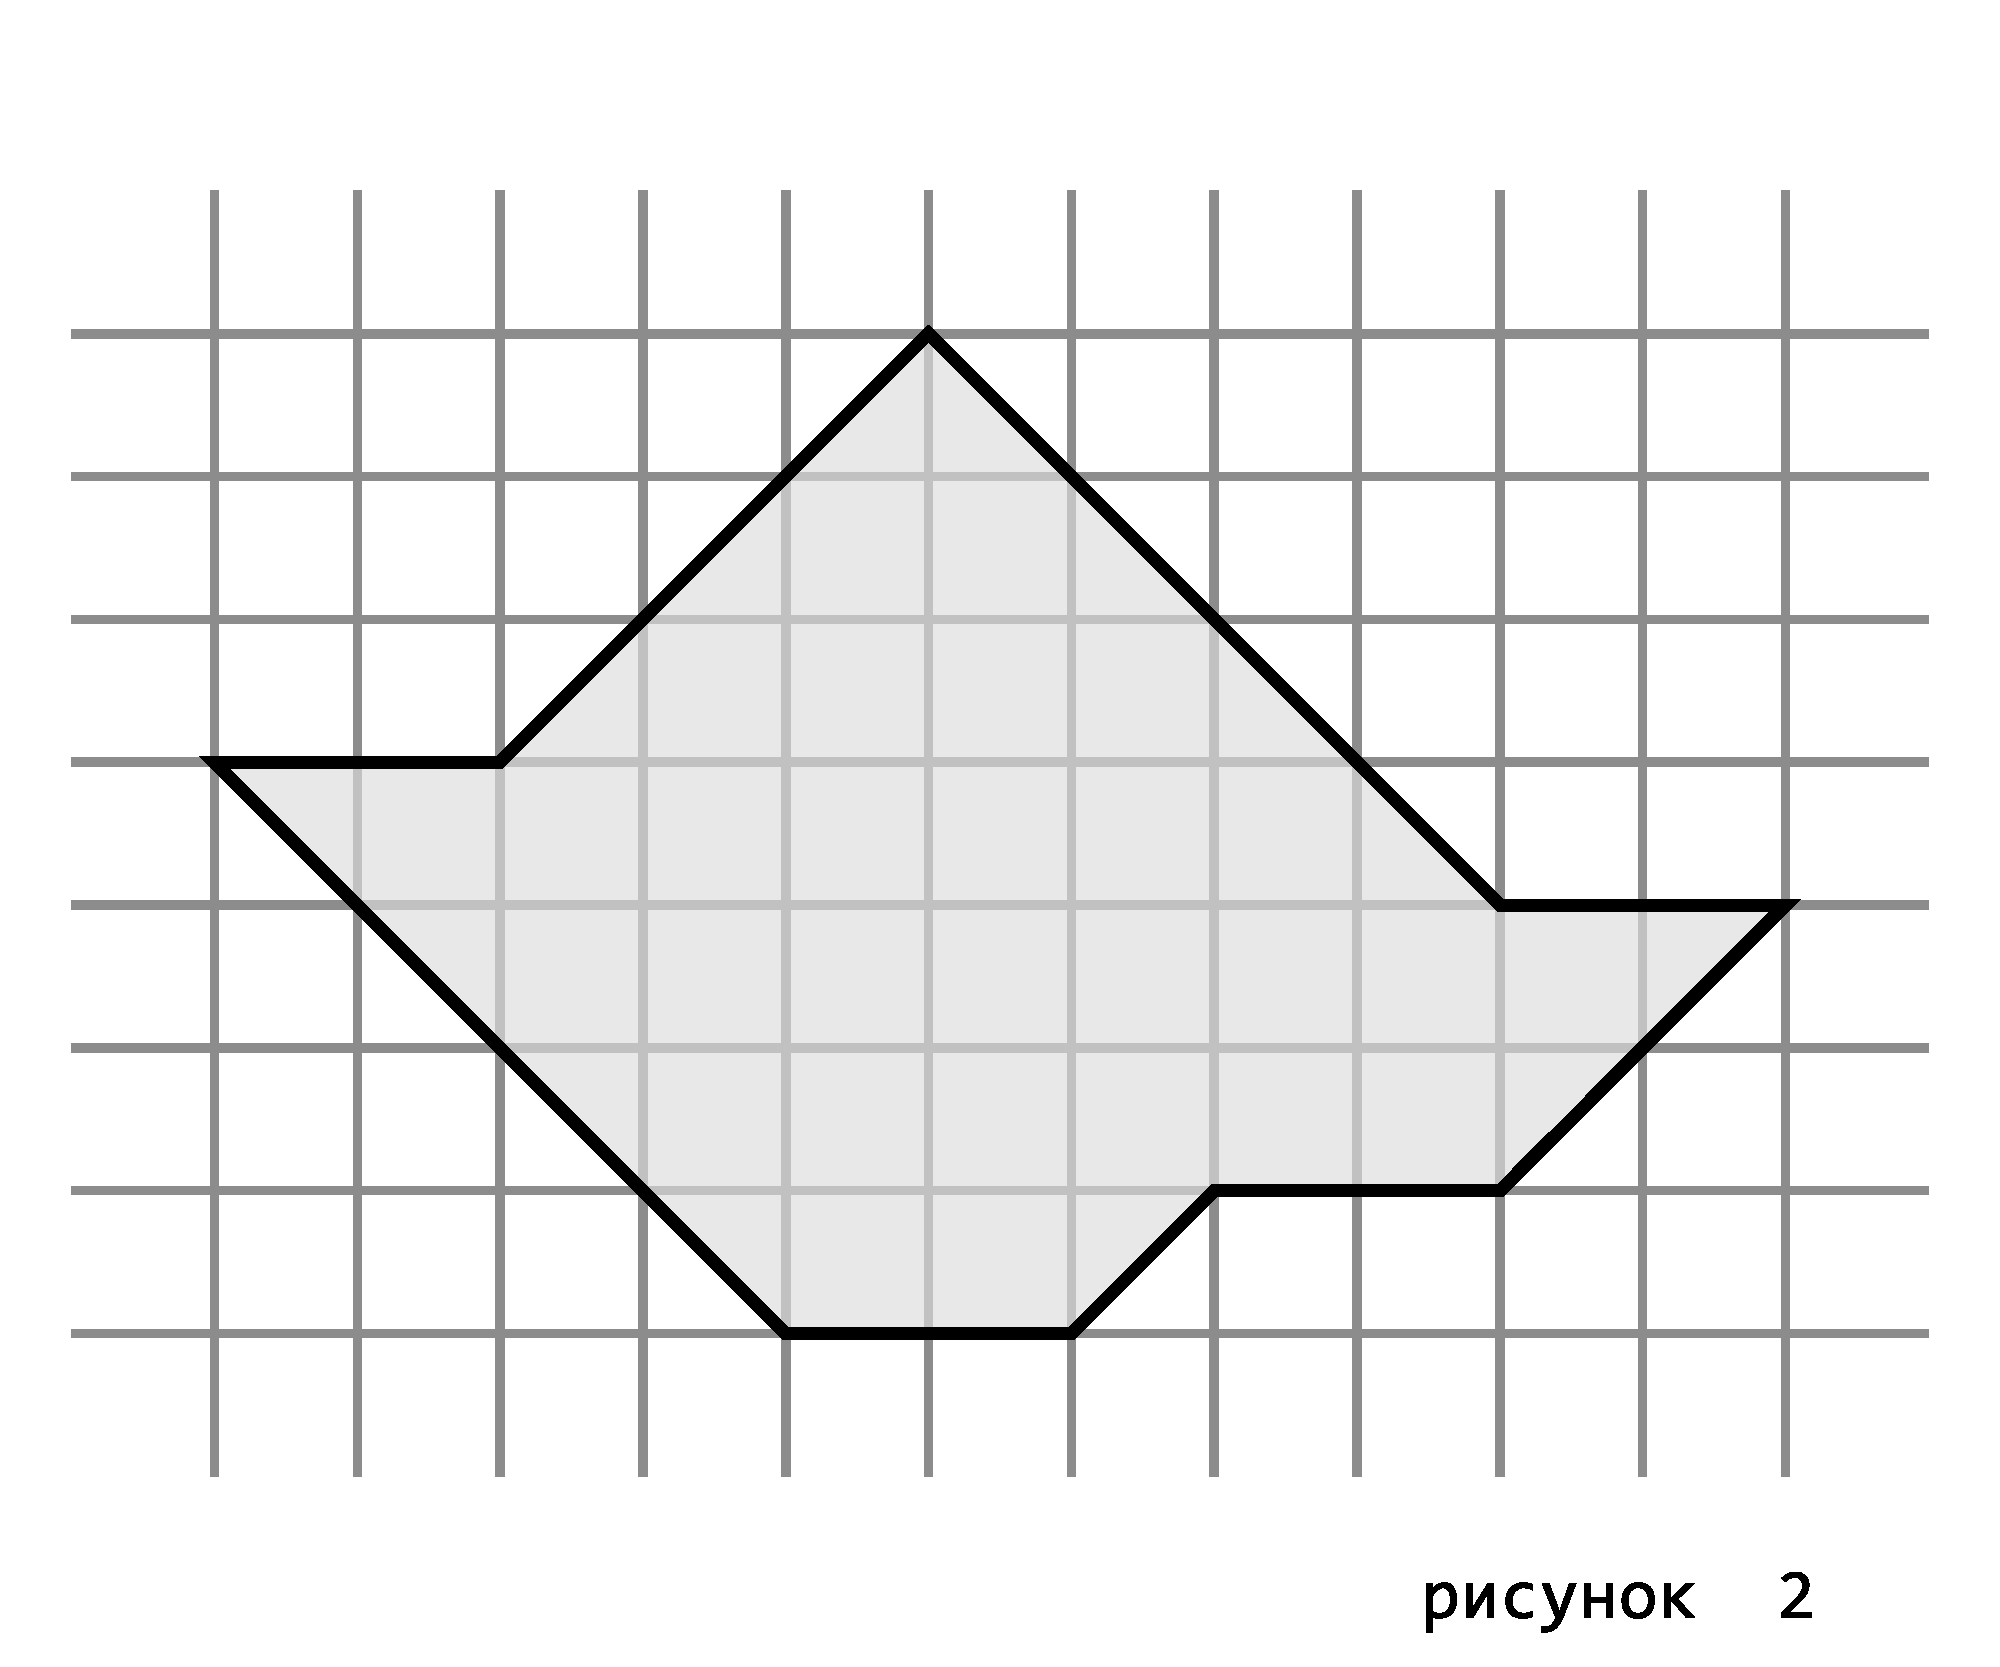
\includegraphics[width=5.5cm]{stats/2018/images/figure-cuts}}

\itC Представьте, что одну из Египетских пирамид (Египетские пирамиды симметричны и имеют в основании квадрат) покрасили розовой краской (покрашены оказались её четыре стороны, но не основание). Как разрезать её на три части одинакового объёма, несущие на себе одинаковое количество краски?
\end{enumerate}